\documentclass[
]{ceurart}

\usepackage[utf8]{inputenc}

\begin{document}

\copyrightyear{2022}
\copyrightclause{Copyright for this paper by its authors.
  Use permitted under Creative Commons License Attribution 4.0
  International (CC BY 4.0).}

\conference{ALTNLP2022: The International Conference on Agglutinative Language Technologies as a challenge of Natural Language Processing, June 6-8, 2022, Koper, Slovenia}

\title{BoAT Web Annotation Tool for Turkish Dependency Parsing}

\author[1]{Furkan Akkurt}[%
email=furkan.akkurt@boun.edu.tr
]

\author[2]{Buşra Marsan}[%
email=busra.marsan@boun.edu.tr
]

\author[1]{Susan Uskudarli}[%
email=suzan.uskudarli@boun.edu.tr
]

\address[1]{ Department of Computer Engineering, Bogazici University, Istanbul, Turkey }
\address[1]{ Department of Linguistics, Bogazici University, Istanbul, Turkey }

\begin{abstract}
The value of quality treebanks is steadily increasing due to the important role they play in the development of natural language processing tools.
The creation of such treebanks is enormously labour-intensive and time consuming.
Therefore, tools that support the annotation process are very valuable.
This is especially the case for morphologically rich languages.
The \boat{} annotation tool was developed for annotating dependency relations, which was used to create the manually annotated \bountreebank{} (UD\_Turkish-BOUN) of Turkish National Corpus (TNC).
The extensive annotation experience revealed several opportunities of improvement.
Combined with our desire to create a multi-user web based annotation tool, this led to the development of \boat{} v2.
The main objectives of the new tool are to: (1) provide further support for creating valid and consistent annotations, (2) significantly improve the user experience of the annotator, and (3) develop an open source and easily deployable web-based annotation tool and an API to benefit the scientific and education community.
This paper discusses the requirements, design, implementation of \boat{} v2 with annotation examples that highlight the new features.
\end{abstract}


\begin{keywords}
natural language processing \sep
linguistic annotation \sep
annotation tool \sep
web application \sep
dependency parsing \sep
Universal Dependencies
\end{keywords}

\maketitle

\section{Introduction}
\label{sec:introduction}

Treebanks are important resources in the development of natural language processing tools.
Quality tools need treebanks that are manually annotated by linguistic experts. 
This is especially true for agglutinative languages due to their complex morphologies. 
The creation of such treebanks is highly labor-intensive and time-consuming due to the meticulous attention required.
Thus, tools that support this process are very important.

% may need a better segue
In recent years, there have been significant efforts to bridge the gap in data resources available for agglutinative low-resource languages.
%Among them is the creation of quality annotated data resources.
Unfortunately, annotation tools developed for analytical languages~\cite{UD} are not to be well suited for agglutinative languages with their complex morphology.
The annotation of agglutinative  languages requires significantly more operations, such as entering several features for each lemma and sometimes even for split lemmas.
Annotation tools that rely on drag-drop and mouse-based interfaces, which seem appealing, are not suitable when entering numerous features is necessary since swapping between input modalities disrupts the flow of concentration.

\boatvone~\cite{turk2021resources} is an annotation tool that was developed to support the dependency annotation of MRLs to produce treebanks compliant with the Universal Dependency framework~\cite{UD}.
It is a standalone application developed using Python and Qt for the user interface.
Its main input modality is via the keyboard on request of the annotators. 
It was used to create the \bountreebank~\cite{turk-etal-2019-turkish,turk2021resources,UD-Boun-Treebank} -- a manually annotated Turkish dependency treebank comprising of thousands of sentences.
This experience revealed several points of improvement for such annotation tools.
% Note: logically doesn't flow after previous statmement. Also, efficiency of a keyboard-oriented approach over an approach of switching between mouse and keyboard was validated in the aforementioned annotation work.
The main takeaway was a much better understanding of the time, effort, cognitive load, and extra information requirements of the annotation process.
Improvements regarding these aspects should, consequently, produce higher quality data resources.

This work presents a dependency annotation tool (\boatvtwo) that has been designed based on the experience with \boatvone.
The design and implementation of the tool aimed to: (1) support the creating valid and consistent annotations with increased speed, (2) significantly improve the user experience of the annotator, (3) allow collaboration among annotators during the annotation process, and (4) provide an open source and easily deployable web-based annotation tool with an API to benefit the scientific community.
The development started with requirements elicitation, for which earlier experiences and in-depth interviews with an experienced annotator were taken into account.

\boatvtwo\ is a web-based collaborative dependency annotation tool that focuses on the user experience of annotators. 
It has and application programming interface (API) for programmatic access and extensibility. 
The tool is dockerized in to facilitate accessibility and ease of  deployment.
The current prototype is being evaluated with positive feedback.
The final version will be made available on the Boğaziçi University's NLP platform~\cite{DIP} and provided as an open source resource.
% This is better in Requirement section. This feedback indicated that the ability to collaborate within the tool is needed to increase efficiency of multi-annotator treebank creation.
% Requirements In light of the feedback, we developed a web application that supports multiple users to enable a collaborative environment for annotations.
% An API was designed to render the functionalities accessible to various NLP applications.
%Several user experience improvements were implemented in order to facilitate the flow of an annotation session.
The main contributions of this work are:
\begin{itemize}
\setlength\itemsep{0em}
        \item Design of a dependency annotation tool that is based on requirements elicited from experienced annotators who are linguists,
        \item The development of a tool that takes into account the annotator experience to improve resulting annotations,
        \item Support for multi-users to provide indivual spaces for annotations, computation of inter-annotator agreements, and other potential collaboration,
        \item The development of a web-based annotation tool based on a supporting API, and
        \item Packaging of the tool to support easy access by virtualizing it using Docker and providing the code as an open source resource.
\end{itemize}

The remainder of this paper is organized as follows:
Section~\ref{sec:related} presents related work,
Section~\ref{sec:requirements} describes the requirements elicitation process and design,
Section~\ref{sec:implementation} presents the implementation with emphasis on the new features,
Section~\ref{sec:annotation} presents a use case of annotation.
We discuss our experiences and point out some future work in Section~\ref{sec:discussion} and offer our conclusions  in Section~\ref{sec:conclusion}.

\section{Related Work}
\label{sec:related}

Annotation tools may be characterized in terms of their accessibility and the support they provide for languages, various annotation categories, user interface modalities, standards, and multiple annotators.
Adherence to standards is recommended to get the most benefit from the annotated data sources.
Universal Dependencies~\cite{UD} is an actively growing standard that intends to cover all languages and its support for agglutinative languages is evolving.

Several dependency annotation tools have been proposed such as \textit{brat}~\cite{brat}, \textit{UD Annotatrix}~\cite{tyers-etal:2018} and \textit{DgAnnotator}~\cite{dgannotator,UD-tools}.
These tools are not developed for a specific language, but can be used with a variety of languages.
They mostly rely on mouse-based user interaction, which is inefficient for annotating agglutinative languages due to the need for extensive annotation for most tokens.

The ITU Treebank Annotation Tool~\cite{pamay-etal-2015-annotation} was developed for Turkish and has been used to annotate the ITU Web Treebank~\cite{itu-web-tb}.
It was written in Java as an open-source standalone tool and has several versions.
It has 3 three stages of annotation: morphological analysis, morphological disambiguation and syntax analysis.
It offers semi-automated support for annotators through analyzers for creating new datasets as well as correcting already existing Turkish treebanks.
It mostly relies on mouse-based interactions and doesn't support the \ud\ framework.

WebAnno~\cite{webanno} is a web-based open-source annotation tool, that is not restricted to dependency annotations but has support for morphological, syntactical, and semantic annotations also, with multi-user support.
To annotate features of a token, it requires several mouse clicks which is impractical for MRLs.
It does not display a dependency graph, unlike \boatvone\ and \boatvtwo.
It presents several sentences simultaneously, which can be distracting.

\boatvtwo\ is the second iteration of \boatvone.
It improves on it by including a search functionality, a database to represent sentences in a more essential way rather than a plaintext file and an accessible web interface with an API for flexibility.
\boatvtwo\ has been developed to reduce clutter that \boatvone\ was found to have in some spaces by the feedback of \boatvone.

\section{Requirements and Design}
\label{sec:requirements}

% Suzan, introduction sentence
In-depth interviews and requirements elicitation with annotators that have annotated the entire \bountreebank{}, which has close to 10 thousand sentences, have been conducted to elicit the software requirements.
Annotators may struggle with a specific annotation and want to be able to search for specific annotations similar to the one they are currently doing to make the treebank consistent within itself and reduce their cognitive load in general.
Thus, a search functionality for annotators needs to be built with a network of annotators to allow them to cross-check each other's work.
Because there was a pressing need for a network, we decided to develop a new web-based tool from scratch.

The annotation process requires a great deal of attention, therefore, the main priority is to improve the user experience for the annotator so that they can more efficiently produce accurate annotations.
Annotators use the tools sometimes for hours on end.
Software should make the work easier by reducing distractions and automating work that can be automated.
One of the requirements we have gathered for not breaking the focus of the annotator is for the software to use only keyboard for every task.
\boat{} is a keyboard-oriented application.
User should not have to use a mouse for any type of task.
Since users lose focus after some time naturally, automating the entries and checking errors are high priorities in this respect.
Autocomplete should be provided for parts of the annotation where it is known what values are allowed for a \conllu{} type annotation.
Autocompletion reduces errors and increases efficiency.

One feature requested by annotators is using the screen space in a compact manner and removing any clutter that's not used much.
Considering this, the previous application's checkboxes have been converted into a dropdown menu, leaving more space for the annotation table where most of the annotator focus is directed towards.

A search API for the annotation database of the treebanks is another requirement.
An annotator should be able to search the treebank they are a part of to see other annotations done for a specific sentence or go to a sentence's annotation page to start annotating.
Sometimes a user may not be sure of an annotation and would like to consult previous annotations for similar cases.
They should be able to search the database in a complex way, by case, features or direct text, etc.
An outsider also should be able to use the API to get the annotations of a particular treebank to use in their tasks in a systematic way.

Following good software practices, this tool should be dockerized and made available as open source.

\section{Implementation}
\label{sec:implementation}

Web application development framework \textit{Django}~\cite{django}, Web API toolkit \textit{Django REST Framework} (DRF)~\cite{drf} and Python~\cite{python} library \textit{django-filter}~\cite{django-filter} are used to operate \boatvtwo.
PostgreSQL~\cite{psql} is used to provide a database for the server-side applications of the software.
During the implementation phase, decisions regarding models of the database have been directed towards the UI utilizing the API for database queries and searches.
The models reflect the \ud\ format of sentences and annotations are saved as fields of word lines.

All the pages of the tool have been supported by Bootstrap~\cite{bootstrap}.
The annotation page has most of the functionalities of \boatvone.
Entries are validated and errors are displayed on the annotation page for annotators to see invalid edits in real time, according to the \ud\ framework~\cite{UD} and the language provided.

Python library \textit{spa\textsc{C}y}~\cite{spacy} is used to provide linear dependency graphs.
Another JavaScript-based linear dependency graph~\cite{spyssalo} making use of \textit{brat}~\cite{brat} is used to provide graphs as well.
An annotator's preference regarding this may vary, thus, giving them visualization options is important.

\begin{figure}[tbh]
    \centering
    \frame{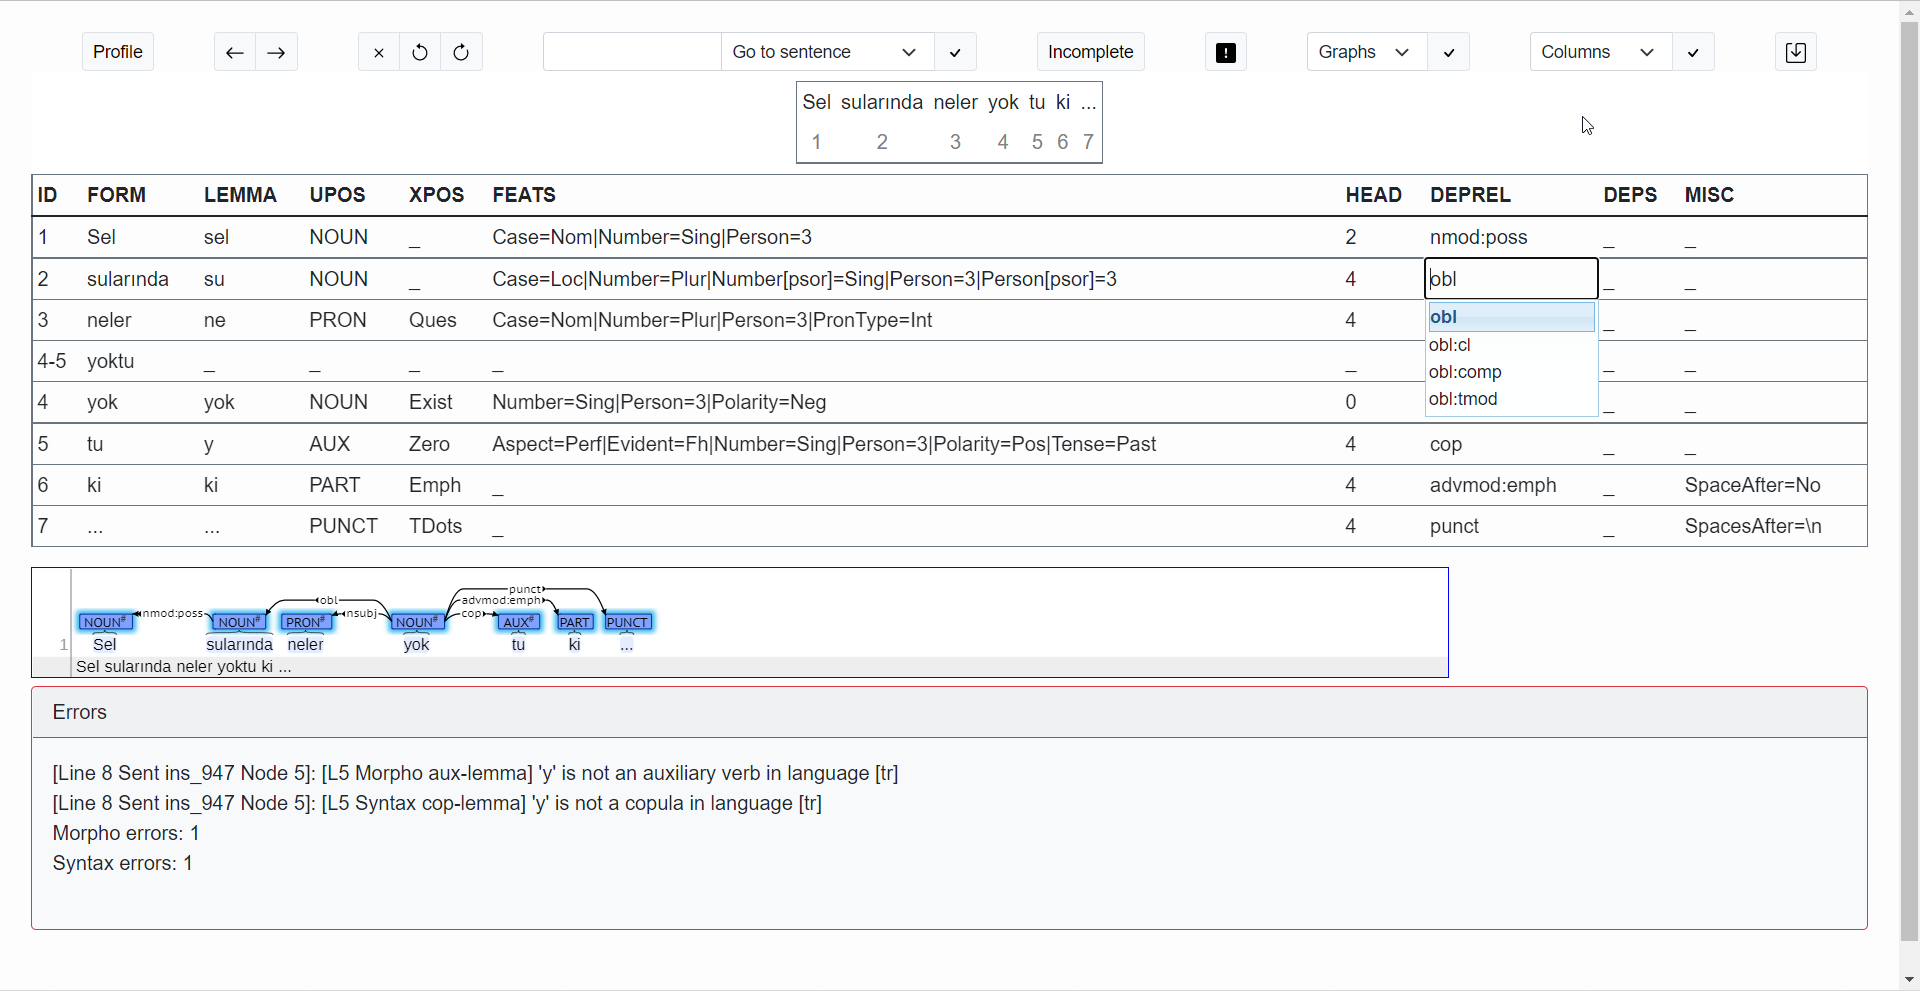
\includegraphics[width=1\textwidth]{figures/sample-annotation.png}}
    \caption{The annotation screen for the sentence ``Sel sularında neler yoktu ki...''.
        The annotator is choosing an annotation for the \deprel\ tag of the \form\ ``sularında''.
        The valid alternatives pop up based on the entry and can be selected via use of arrows. }
    \label{fig:anno-fig}
\end{figure}

\subsection{Features}
\label{sec:features}

There are many new features and improvements in this tool, as well as most of the functionality of \boatvone.

\begin{itemize}[before=\normalfont, font=\itshape, align=left]
    \item[Treebanks:]
        Multiple treebanks, with each one having its own sets of sentences, can be created in a single deployment.
        When uploading a file, a treebank is selected.

    \item[Loading files:]
        Instead of loading a dataset file before every annotation session, a \conllu\ file is uploaded to the database.
        The file is rejected if incorrectly formatted, otherwise uploaded to the database.
        This way, other annotators working with the same treebank don't have to provide the same file.

    \item[Annotation view:]
        The annotation page is very similar to the one on \boatvone~\cite{trk2020resources}, as seen in Figure~\ref{fig:anno-fig}.
        There is an annotation table for annotating fields in word lines of sentences.
        It also includes a dependency graph and an error card, both of which are in sync with the edits done on the table cells.
        Three different dependency graph representations are provided in this tool.
        Two of the graphs, which are both horizontal and linear, have been selected due to space considerations.
        The error card displays errors for the current annotation, validating it via the UD validation script.

    \item[Network-enabled search:]
        An important feature in this version is the ability to cross-check annotations by implementing a network for annotators where they can review the annotations done by other annotators.
        This can be helpful and a learning experience for annotators.

        For example, the annotator of the \bountreebank was annotating a sentence with a Zodiac sign noun.
        Not being sure of how to annotate its \upos\ tag, she searched the \conllu\ file manually for similar cases and encountered two different values with which nouns of Zodiac signs were annotated previously.
        Besides not helping how to choose a \upos\ tag, this raises a consistency issue within the treebank as well.
        This task could have been handled by a search of the database.
        We provide a search page and an API in this tool with which treebanks can be searched by \ud\ tags.

        Another example could be given by the various \textit{-ki} morphemes in Turkish.
        In the sentence ``Evdeki halılar yıkandı.'' (\textit{The rugs at home were washed.}), the \textit{-ki} acts as an adjectivizer.
        However, in ``Benim halılarım yün, Ayşeninkiler sentetik.'' (\textit{My rugs are woolen. Ayşe's are synthetic.}), it is pronominal.
        An annotator might not recall how a specific \textit{-ki} morpheme should be annotated, which can be remedied with a simple search.
        Annotators have informed us that such cases occur frequently when annotating MRLs.

        The inter-annotator agreement allows us to see some anomalies in the Turkish part of the \ud\ framework.
        For example, if a sentence were annotated a way by many annotators but the \ud\ validation script were finding it invalid, this might indicate the validation were lacking in this respect of the Turkish language.

    \item[Annotation status:]
        There are 3 annotation statuses ("Incomplete", "Draft" and "Complete") and they are cycled through by the annotator in the annotation view.
        Status of an annotation is also shown in the search view, helping to select an appropriate case.
        There is another view where completed, drafted or incomplete annotations can be listed.

\end{itemize}

\section{Features}
\label{sec:features}

There are many new features and improvements in this tool, as well as the functionality that already existed in BoAT v1.
Instead of loading a specific file before annotating, a user is able to upload a \conllu{} file to the database and start annotating.
The file is parsed and checked for its format. It's rejected if incorrectly formatted, then uploaded to the database.
This way, other annotators working for the same treebank don't have to provide the same file.

The annotation page is very similar to BoAT v1.
It includes a dependency graph and an editable table, both of which in sync.
The dependency graph of the initial tool and other 2 graphs have been added to this tool.
The user has the choice to select a type of graph or none.
The other 2 graphs, which are both horizontal and linear, have been selected due to space considerations.
The annotation table is for editing the word lines of \conllu{} files.

An important feature in this version is the ability to cross-check annotations by implementing a network for annotators where they can see the annotations done by other annotators and if they disagree on some parts, they can interact outside the tool.
This can be helpful and a learning experience for annotators.
For an actual example, the annotator, responsible for the BOUN Treebank's annotation, was annotating a sentence that had a Zodiac sign noun.
Not being sure about how to annotate the noun's dependency relation, she searched for similar cases in the \conllu{} file and encountered two different ways nouns of Zodiac signs were annotated previously.
Beside not helping how to choose a \textit{UPOS} tag, this raises a consistency issue within the treebank as well.
For an example of a Turkish sentence with a noun for a Zodiac sign, in the sentence "Terazi rahatına düşkündür." (\textit{"Libras like comfort."}), "Terazi" was annotated as \textit{NOUN} in its \textit{UPOS} tag.
In another sentence "Yükselen Başak düzeni sever." (\textit{"Virgo Rising likes order"}), "Başak" was annotated as \textit{PROPN} in its own \textit{UPOS} tag.
In a similar case, the annotator searched the \conllu{} file in a text editor and decided to use the one with the more cases of annotation and proceeded to replace the inconsistent ones with the decision.
This case can be handled by a simple search of the database.
We provide a search page and its API in this tool where treebanks can be searched by \textit{sent_id}s, \textit{text}s, all the UD tags and treebank names.
With this, an annotator can easily make the treebank more consistent.

% ki example
% Evdeki halılar -> adjectivizer ki 
% Benim halılarım yün, Ayşeninkiler sentetik. -> pronominal 

Also one other thing the interannotator agreement allows us is the possibility to see some anomalies in the Turkish part of the validation of the UD framework.
For example, if a sentence were annotated a way by many annotators but the UD validation script were finding it invalid, this might indicate the UD validation were lacking in this respect of the Turkish language.
Some modifications might be necessary and there could be a case for a proposal of change.

\section{Annotation Procedure}
\label{sec:annotation}
This section describes how an annotator annotates a Turkish sentence.

An annotator selects a sentence from a treebank, which has previously uploaded sentences coming from a \conllu{} formatted file.
They fill the cells of the annotation table's fields.
During the annotation, an annotator can make use of dependency graphs, error cards and the search functionality.
Dependency graphs are visual cues for how an annotation is going, using HEADs and DEPRELs.
They can choose 3 different graphs one at a time or select to hide.
Different graphs show the same information with a horizontal or vertical tree.
Errors are helpful reminders, coming from a validation script found on the UD repository.
They can use the search functionality to search for previous annotations by other annotators or themselves, using various fields (text, FEATS, etc.) for the query.
By checking similar annotations, an annotator can ensure consistency and don't lose focus by trying manual methods for the same information.
When an annotation is done, they select the annotation to be "Complete".

\section{Discussion and Conclusions}
\label{sec:discussion}

% subsections are needed ; for example, for testing
\todo[inline]{subsections are needed ; for example, for testing}

\boatvtwo\ aims to extend the functionality of \boatvone\ as a collaborative web-based application to support the annotation process based on previous experiences.
We developed a web application that supports agglutinative languages as described in Section~\ref{sec:implementation}.

The implementation choices served our goals well.
We believe that having experts in linguistics and experienced annotators in agglutinative treebank creation was instrumental in understanding the requirements and the design process.
We held numerous elicitation interviews and further meetings for clarifications and feedback requests.

We used modern software development tools and management practices during the development lifecycle of this tool.
The development of an API enables various extensions of this tool and access to the treebanks.
The containerization with Docker~\cite{docker} has facilitated easy delivery and deployment.
It is available on Boğaziçi University's NLP platform~\cite{TULAP} as an open-source resource.
The availability of the tool as a user as well as a developer is valuable for future use and developments.

% we've done some testing ; more testing and documentation here would be useful
This tool is in the testing phase and has had encouraging early feedback.
We compared the annotation of several sentences with the same number of tokens using \boatvone\ and \boatvtwo.
While we kept the number of words in a sentence constant, we did not use the same sentences since having previously annotated a sentence would impact the annotation on another version.
Keeping the number of words the same provides a somewhat comparable experience.
There was a noticeable speedup (approximately 30\%) using \boatvtwo.
% above testing need not be mentioned in this paper
Among the new features that are most appreciated are autocompletion, condensed dependency tree representation, significant reduction on scrolling, keyword search, and search by morphological features.
The non-search related features are instrumental to retaining focus.

We are encouraged by the early responses to this tool and anticipate its extensions.
In fact, our implementation of \boatvtwo\ resulted in a revision request for \boatvone\ to include the focus enhancing features.
This also resulted in significant speedup and improved user experience, which was reported as a qualitative observation by an annotator.
Presently, our testing is focused on more extensive cases (annotation of sentences with varying degrees of complexity) and, importantly, the multi-user functionalities.
For this purpose, we are in the process of recruiting several annotators with a background in linguistics.


\section{Conclusion}
\label{sec:conclusion}
% with boat feedback, web version planned
% dockerized, implemented
% we believe it's helpful
% nlp website accessible

\begin{acknowledgments}
This work was supported by Boğaziçi University Research Fund Grant Number 16909.
\end{acknowledgments}

\bibliography{main}

\end{document}
